\section{BMS Software}
Text

\subsection{Design}
text\\

\textbf{Din text her} \\
\\
The BMS software is programmed to the Digital Unit. The purpose of the BMS software is to continually collect data from the Analog Front End and then inspect this data to see if the batteries are working as expected. Data is at least collected every second, but if the collected data has parameters close to the respective threshold, the data collection increases to being done every 200 milliseconds, where also a safety check of the parameters is executed. \fxnote{Reference to 2013BMS Documentation function safety\_check()}

This is because it is assumed that if the data is far away from the thresholds, the thresholds are most likely not exceeded as quick as if the data was close to the thresholds. It is very important to have a safe operating system with many safety checks, but it is also important to do as few calculations as possible. This is because the system should be in the power saving “sleep mode” as much of the time as possible to save energy and thereby be as energy efficient as possible.

If the battery cells at startup has a voltage too high, the BMS system sets the cells to balance down in voltage with the help of bleeder resistors and sets the initiation of the system on a hold for four seconds, so that the cells have time to discharge. The twelve cells are also analyzed every second, so that if any threshold is exceeded, the isolation switch is opened, and will stay this way until the cells are balanced back within acceptable thresholds. This balancing is possible when a charger is connected. Lastly every second the collected data is send via CAN-Communication. After 20 seconds have passed, a State Of Charge analysis (SOC-analysis) is executed, this data is of course also send via CAN\_Communication.

Details about how the software works can be found in BAC….\fxnote{Reference to 2013BMS Documentation} Where the software is well documented with flowcharts, application models/class diagrams and function descriptions.
The BMS software consists of the following c- and h-files:\\
\begin{figure}[H]
	\centering
	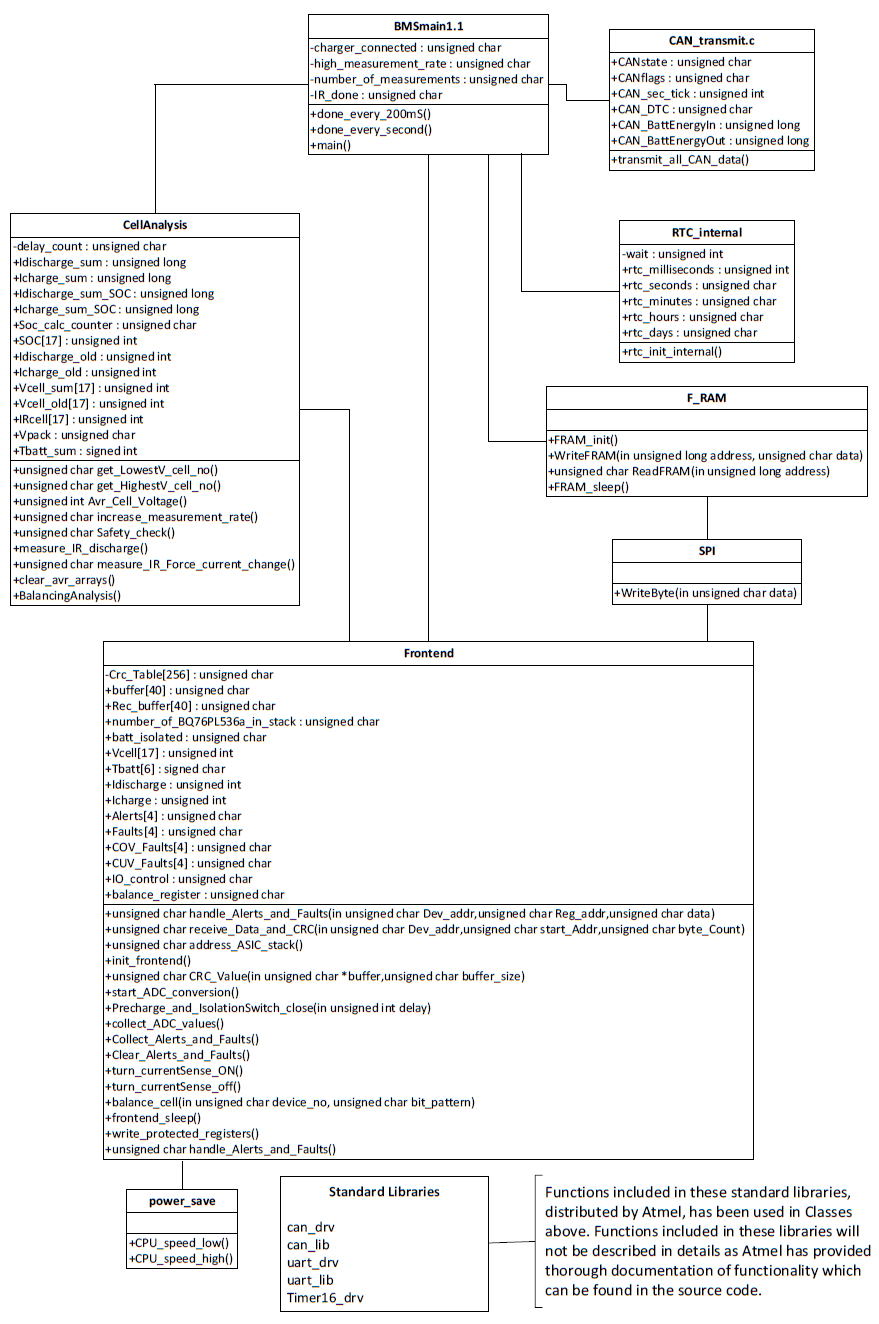
\includegraphics[width=1.0\linewidth]{Software/BMS-ClassDiagram.PNG}
	\caption{Class Diagram from 2013BMS Documentation}
	\label{fig:SOFTWARE_BMS}
\end{figure}
The only function description that isn’t documented is the “CalculateSOC()” function. This is because “CalculateSOC()” was re-implemented as a function in 2014 instead of just being part of the “done\_every\_second()” function. Therefore the function description for the “CalculateSOC()” will be presented now. (This function is located in the CellAnalysis.c file):
\begin{table}[h!]
	\centering
	\label{CalculateSOCfunction}
	\begin{tabular}{|p{4 cm}|p{9 cm}|}
		\hline
		\textbf{Function:} & \textbf{void CalculateSOC(void)}	\\\hline
		Parameters	& None	\\\hline
		Return Value	& None	\\\hline
		Description of function	& After data has been collected this function can be called and the state of charge will be found by compared the value of the cell voltages and ten different levels of voltage. This way the state of charge will be represented from 1 to 10, where 1 is 10 percent and 10 is 100 percent.	\\\hline
	\end{tabular}
	\caption{function description of the CalculateSOC function}
\end{table}

\textbf{END OF DIN TEXT} \\ 
\\


\subsection{Implementation}
text

\subsection{Unity test}
text